\chapter{费米子、狄拉克矩阵与狄拉克海}

狄拉克海是我们的目的地，但路径很重要。在相对论性电子理论中面对负能量之前，我们需要两件工具。首先是区分费米子与玻色子的算符代数。然后是对一维狄拉克方程的回顾，在那里波函数的每一次扩大都可以被看清，而不必借助三维空间的几何。一旦这些工具就位，三维方程将迫使其自身的矩阵结构出现，而关于被占据与空着的费米子态的开篇讨论将作为理解正电子的关键回归。

我们使用\(c=\hbar=1\)。大写\(P\)表示动量算符，小写\(p\)表示动量本征值，粗体符号表示它们的三维版本。

\section{交换变为算符代数}

考虑两个全同粒子，一个在\(x\)处，一个在\(y\)处。标记\(x\)和\(y\)表示完整的位置；它们不是单个粒子的两个笛卡尔坐标。用两个产生算符作用于真空给出
\begin{equation}
\lvert x,y\rangle
=
\psi^\dagger(x)\psi^\dagger(y)\lvert0\rangle.
\label{eq:l10-two-particle-state}
\end{equation}

对于玻色子，交换这两个位置不改变态：
\begin{equation}
\lvert x,y\rangle=\lvert y,x\rangle.
\end{equation}
保证这一对称性的算符陈述是
\begin{equation}
\psi^\dagger(x)\psi^\dagger(y)
=
\psi^\dagger(y)\psi^\dagger(x).
\label{eq:l10-boson-exchange}
\end{equation}
两个玻色子产生算符对易，因此我们可以颠倒它们的顺序而不改变它们所产生的态。

对于费米子，交换改变符号：
\begin{equation}
\lvert x,y\rangle=-\lvert y,x\rangle.
\label{eq:l10-fermion-state-exchange}
\end{equation}
孤立态矢量的整体符号不可观测，但不同备选之间的相对符号是可观测的，因此这个负号必须被一致地携带。方程~\eqref{eq:l10-fermion-state-exchange}要求
\begin{equation}
\psi^\dagger(x)\psi^\dagger(y)
=
-\,\psi^\dagger(y)\psi^\dagger(x).
\label{eq:l10-fermion-operator-exchange}
\end{equation}

\begin{figure}[htbp]
\centering
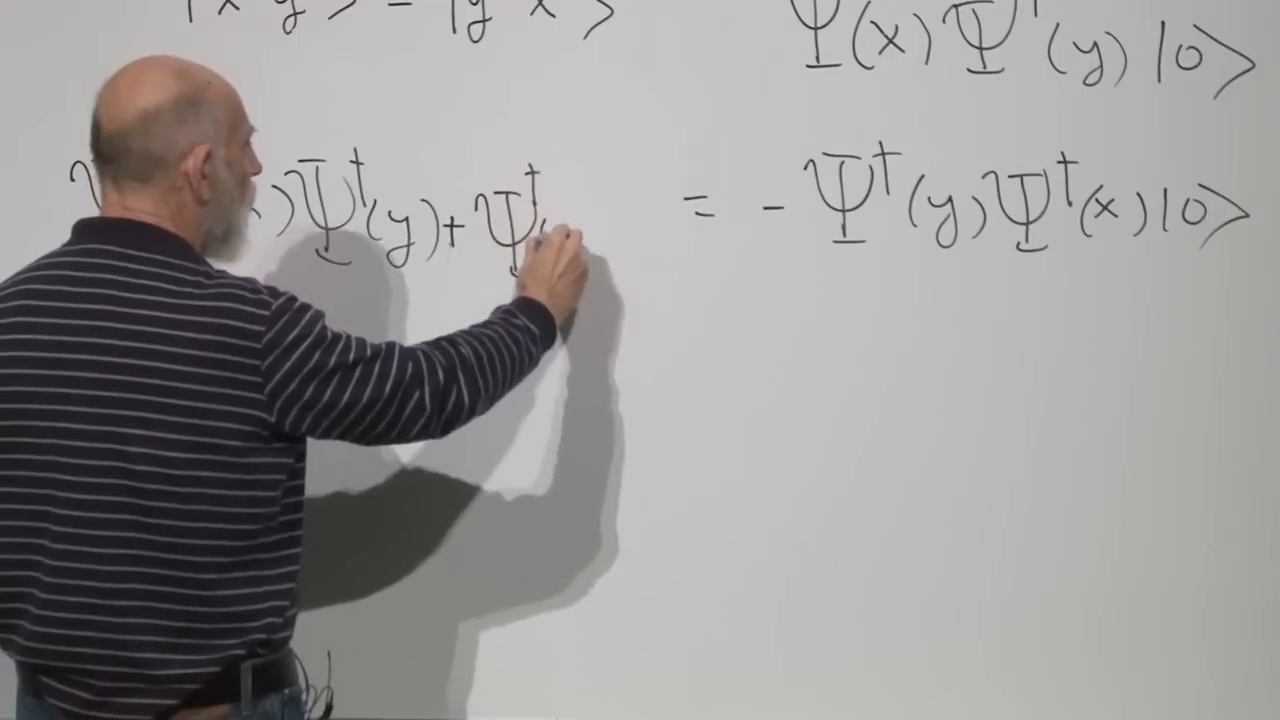
\includegraphics[width=0.94\linewidth]{lecture_10_figure_02.png}
\caption{黑板上实现费米子交换的关系。交换产生算符会反转两粒子态的符号。}
\lectureframe{00:05:50}
\end{figure}

对于任意两个算符\(A\)和\(B\)，定义反对易子为
\begin{equation}
\{A,B\}:=AB+BA.
\end{equation}
因此交换规则为
\begin{equation}
\{\psi^\dagger(x),\psi^\dagger(y)\}=0.
\label{eq:l10-creation-anticommutator}
\end{equation}
相应的费米子场代数将玻色子对易子替换为反对易子。必须区分这个词的两种用法：场算符反对易是因为费米统计，而矩阵稍后将反对易，以便在相对论性色散关系中抵消交叉项。

现在在式~\eqref{eq:l10-creation-anticommutator}中令\(y=x\)。两个乘积变得相同：
\begin{align}
0
&=\{\psi^\dagger(x),\psi^\dagger(x)\}\\
&=2\,\psi^\dagger(x)\psi^\dagger(x).
\end{align}
因此
\begin{equation}
\bigl(\psi^\dagger(x)\bigr)^2=0.
\label{eq:l10-exclusion}
\end{equation}
试图在同一单粒子态中产生两个同种的费米子，会得到零矢量。这就是用算符表示的排他原理。

\begin{figure}[htbp]
\centering
\includegraphics[width=0.94\linewidth]{lecture_10_figure_03.png}
\caption{黑板上对相同态的特化。重复的产生算符乘积出现两次，因此必须为零。}
\lectureframe{00:08:04}
\end{figure}

\begin{figure}[htbp]
\centering
\begin{adjustbox}{max width=\linewidth}
\begin{tikzpicture}[node distance=1.25cm,>=Latex]
\node[draw,rounded corners,align=center,inner sep=7pt] (a)
  {$\{\psi^\dagger(x),\psi^\dagger(x)\}=0$};
\node[draw,rounded corners,align=center,inner sep=7pt,right=of a] (b)
  {$2(\psi^\dagger(x))^2=0$};
\node[draw,rounded corners,align=center,inner sep=7pt,right=of b] (c)
  {$(\psi^\dagger(x))^2=0$};
\draw[->,thick] (a) -- (b);
\draw[->,thick] (b) -- (c);
\end{tikzpicture}
\end{adjustbox}
\caption{在不借助部分擦除的中间黑板工作的情况下重建的不相容性论证。}
\end{figure}

\section{为什么对费米子而言被占据与空着是对称的}

玻色子与费米子算符之间还有第二个区别，比不相容性更微妙，且对后续至关重要。对于单个玻色子模式，
\begin{equation}
[a,a^\dagger]=1,
\qquad
n=0,1,2,\ldots.
\end{equation}
交换\(a\)和\(a^\dagger\)会改变对易子的符号。即使这些算符仅仅被称为\(A\)和\(B\)，代数也会告诉我们哪种顺序提高占据数，哪种顺序降低它。

玻色子占据阶梯也有方向。湮灭算符最终到达\(\lvert0\rangle\)并给出零，而产生算符可以无限继续：
\begin{align}
a\lvert0\rangle&=0,\\
a^\dagger\lvert n\rangle&\propto\lvert n+1\rangle,
\qquad n=0,1,2,\ldots.
\end{align}
把这个阶梯上下颠倒不会重现相同的谱。有一个底但没有顶。

对于一个费米子模式，
\begin{equation}
\{a,a^\dagger\}=1,
\qquad
a^2=(a^\dagger)^2=0,
\qquad
n=0,1.
\label{eq:l10-fermion-mode}
\end{equation}
产生算符把空态变为满态，然后停止：
\begin{equation}
a^\dagger\lvert0\rangle=\lvert1\rangle,
\qquad
a^\dagger\lvert1\rangle=0.
\end{equation}
湮灭算符执行相反的操作：
\begin{equation}
a\lvert1\rangle=\lvert0\rangle,
\qquad
a\lvert0\rangle=0.
\end{equation}
只有两个态，因此该图在交换满与空以及交换\(a\)与\(a^\dagger\)之下是对称的。这些算符仍然具有不同的物理意义，但它们的代数不再把其中一个单独挑出为产生、另一个为湮灭。这种形式对称性是粒子-空穴重新解释的种子。

\begin{classroomqa}
\lecturetimestamp{00:13:54}
\audiencequestion{如果\((a^\dagger)^2=0\)，那是矛盾，还是意味着\(a^\dagger=0\)？}
\lecturerresponse{都不是。一个非零算符可以有为零的平方。这里\(a^\dagger\)把\(\lvert0\rangle\)变为\(\lvert1\rangle\)，但在\(\lvert1\rangle\)之上没有允许的态，因此对它作用两次给出零。同样的推理给出\(a^2=0\)。}
\end{classroomqa}

把这种填满-空位的对称性留作备用。当移走一个负能量电子时，湮灭算符将被重新标记为正电子产生算符。这一操作并非任意改变记号；它恰好使用了此处建立的两态费米子代数。

\section{一维狄拉克构造}

现在回到一维空间中的一个粒子。最简单的一阶相对论性波动方程为
\begin{equation}
i\partial_t\psi=-\,i\partial_x\psi.
\label{eq:l10-right-mover}
\end{equation}
其中\(P=-i\partial_x\)，这即为
\begin{equation}
H=P.
\end{equation}
一个动量本征态有\(E=p\)，其群速度为
\begin{equation}
v_g=\frac{dE}{dp}=1.
\end{equation}
正或负的动量，因而正或负的能量，仍然给出刚性向右运动的波。\(p\)的符号改变的是相位图样，而不是传播方向。

一个有质量的粒子必须能够向任一方向运动。引入满足下式的第二个分量
\begin{equation}
H\psi_1=P\psi_1,
\qquad
H\psi_2=-P\psi_2.
\label{eq:l10-two-directions}
\end{equation}
第一个分量向右运动；第二个分量向左运动。把它们放入一个列向量，
\begin{equation}
\Psi=
\begin{pmatrix}
\psi_1\\
\psi_2
\end{pmatrix},
\end{equation}
并定义
\begin{equation}
\alpha=
\begin{pmatrix}
1&0\\
0&-1
\end{pmatrix}.
\end{equation}
两个方程都变为
\begin{equation}
H\Psi=\alpha P\Psi.
\label{eq:l10-massless-one-d}
\end{equation}
包含两个方向的代价是一个新的二值内部自由度。

仅靠方向本身并不产生质量。引入第二个矩阵，
\begin{equation}
\beta=
\begin{pmatrix}
0&1\\
1&0
\end{pmatrix},
\end{equation}
并尝试
\begin{equation}
H=\alpha P+\beta m.
\label{eq:l10-massive-one-d}
\end{equation}
这些矩阵满足
\begin{equation}
\alpha^2=\beta^2=\mathbb{1},
\qquad
\{\alpha,\beta\}=0.
\label{eq:l10-one-d-algebra}
\end{equation}
将哈密顿量平方得到
\begin{align}
H^2
&=(\alpha P+\beta m)^2\\
&=\alpha^2P^2+\beta^2m^2
  +(\alpha\beta+\beta\alpha)Pm\\
&=P^2+m^2.
\label{eq:l10-one-d-dispersion}
\end{align}
式~\eqref{eq:l10-one-d-algebra}中的反对易子消去了同时含\(P\)和\(m\)的多余线性项。

非对角矩阵\(\beta\)耦合两个方向分量。把质量项想象为不断混合右行和左行振幅是有用的。这一图像不应被字面化为粒子沿微观轨道来回弹跳，但它抓住了为什么一个有质量的波包可以具有低于光速的平均速度并可以拥有静止系，而一个孤立的无质量手征分量却不能。

\begin{classroomqa}
\lecturetimestamp{00:23:37}
\audiencequestion{引入两个方向分量是否有更深刻的物理解释？}
\lecturerresponse{有，但它在三维中更清楚地显现出来。在这个阶段，它们只是描述相反传播并允许非对角质量耦合所需的两个分量。它们后来的解释是手性，即手征性。}
\end{classroomqa}

\section{三维迫使泡利矩阵出现}

在三维空间中，动量是一个矢量。因此，一个对动量线性且旋转标量的哈密顿量暗示着另一个矢量，现在是一个其分量为矩阵的矢量：
\begin{equation}
H=\boldsymbol{\alpha}\cdot\mathbf P
=\alpha_xP_x+\alpha_yP_y+\alpha_zP_z.
\label{eq:l10-three-d-ansatz}
\end{equation}

\begin{figure}[htbp]
\centering
\includegraphics[width=0.94\linewidth]{lecture_10_figure_04.png}
\caption{三维无质量假设\(H=\boldsymbol{\alpha}\cdot\mathbf P\)，正处于一个矩阵变为三个矩阵的矢量之处。}
\lectureframe{00:26:00}
\end{figure}

再次从无质量情形开始。我们要求
\begin{equation}
H^2=\mathbf P^2=P_x^2+P_y^2+P_z^2.
\end{equation}
展开式~\eqref{eq:l10-three-d-ansatz}的平方，
\begin{align}
H^2
&=\alpha_x^2P_x^2+\alpha_y^2P_y^2\\
&\quad+\alpha_z^2P_z^2\\
&\quad+\{\alpha_x,\alpha_y\}P_xP_y\\
&\quad+\{\alpha_x,\alpha_z\}P_xP_z\\
&\quad+\{\alpha_y,\alpha_z\}P_yP_z.
\end{align}
如果
\begin{equation}
\alpha_x^2=\alpha_y^2=\alpha_z^2=\mathbb{1},
\end{equation}
则对角项正确，而如果
\begin{equation}
\{\alpha_i,\alpha_j\}=0,
\qquad i\ne j.
\label{eq:l10-alpha-anticommutation}
\end{equation}
则所有交叉项消失。

三个熟悉的\(2\times2\)矩阵恰好做到这一点：
\begin{equation}
\sigma_x=
\begin{pmatrix}
0&1\\
1&0
\end{pmatrix},
\quad
\sigma_y=
\begin{pmatrix}
0&-i\\
i&0
\end{pmatrix},
\quad
\sigma_z=
\begin{pmatrix}
1&0\\
0&-1
\end{pmatrix}.
\label{eq:l10-pauli-matrices}
\end{equation}
因此一个解是
\begin{equation}
\alpha_i=\sigma_i,
\qquad
H=\boldsymbol{\sigma}\cdot\mathbf P.
\label{eq:l10-weyl-hamiltonian}
\end{equation}

\begin{figure}[htbp]
\centering
\includegraphics[width=0.94\linewidth]{lecture_10_figure_05.png}
\caption{紧凑的无质量哈密顿量\(H=\boldsymbol{\sigma}\cdot\mathbf P\)，其中\(\alpha_z=\sigma_z\)仍在其上方可见。}
\lectureframe{00:28:16}
\end{figure}

对于一个动量本征态，
\begin{equation}
\boldsymbol{\sigma}\cdot\mathbf p
=
|\mathbf p|\,\boldsymbol{\sigma}\cdot\widehat{\mathbf p}.
\end{equation}
算符\(\boldsymbol{\sigma}\cdot\widehat{\mathbf p}\)有本征值\(+1\)和\(-1\)，所以
\begin{equation}
E=\pm|\mathbf p|.
\end{equation}
在这个二分量理论中，正能量的泡利自由度与动量同向排列，而负能量的则反向排列。这种排列是被锁定的；对于固定的能量符号，它不是一个可独立调节的自旋方向。

\begin{classroomqa}
\lecturetimestamp{00:30:10}
\audiencequestion{自旋是从狄拉克方程中掉出来的，还是因为电子已知具有磁矩而被插入的？}
\lecturerresponse{这里的“掉出来”意思是“作为结果出现”，而不是“消失”。出发要求是一个对动量线性且其平方为\(\mathbf P^2\)的哈密顿量。普通数无法满足所需的代数，但泡利矩阵可以。因此它们的二分量结构随线性化本身一同到来。这并不证明每个粒子都必须有自旋；它说的是，由这种狄拉克型方程描述的粒子带有相应的旋量自由度。}
\end{classroomqa}

这是该构造的核心教训之一。这些矩阵并非在找到相对论性方程之后添加的装饰性标签。试图对相对论性色散关系取局部平方根，就产生了它们。

\section{为什么质量需要四个分量}

尝试在不扩大\(2\times2\)理论的情况下重复一维质量的构造：
\begin{equation}
H=\boldsymbol{\sigma}\cdot\mathbf P+\beta m.
\label{eq:l10-failed-mass}
\end{equation}
假设\(\beta^2=\mathbb{1}\)。其平方包含所需项\(\mathbf P^2+m^2\)，但它也包含
\begin{equation}
m\sum_i\{\sigma_i,\beta\}P_i.
\end{equation}
为去掉这一项，某个矩阵\(\beta\)必须满足
\begin{equation}
\{\sigma_x,\beta\}
=
\{\sigma_y,\beta\}
=
\{\sigma_z,\beta\}
=0.
\label{eq:l10-impossible-beta}
\end{equation}
没有任何\(2\times2\)矩阵能做到这一点。单位矩阵与三个泡利矩阵都对易，而每个无迹的\(2\times2\)矩阵都是泡利矩阵的线性组合。任何这样的组合都无法与平行于它的分量反对易。\(2\times2\)代数没有所需类型的第四个独立矩阵。

补救办法是扩大旋量。四个相互反对易且平方为单位矩阵的矩阵首次出现在\(4\times4\)复表示中。选择这个矩阵大小并不是因为时空有四维；它是能够实现所需代数的最小矩阵空间。

存在许多等价的表示。旋量基的幺正变换会改变所有矩阵的矩阵元，却不改变任何物理预言。重要的是抽象的关系集合
\begin{equation}
\{\alpha_i,\alpha_j\}=2\delta_{ij}\mathbb{1},
\qquad
\{\alpha_i,\beta\}=0,
\qquad
\beta^2=\mathbb{1}.
\label{eq:l10-dirac-algebra}
\end{equation}

\begin{classroomqa}
\lecturetimestamp{00:37:38}
\audiencequestion{能否把\(\beta\)看作时间分量\(\alpha_t\)？}
\lecturerresponse{不能直接这样看。三个\(\alpha_i\)并不与\(\beta\)组合成一个洛伦兹矢量的四个分量。在协变记号中，人们改为定义\(\beta=\gamma^0\)和\(\alpha_i=\gamma^0\gamma^i\)；四个\(\gamma^\mu\)矩阵满足时空克利福德代数。}
\end{classroomqa}

一个方便的分块表示为
\begin{equation}
\alpha_i=
\begin{pmatrix}
\sigma_i&0\\
0&-\sigma_i
\end{pmatrix},
\qquad
\beta=
\begin{pmatrix}
0&I_2\\
I_2&0
\end{pmatrix}.
\label{eq:l10-block-representation}
\end{equation}
对角块中的泡利矩阵保证不同的\(\alpha_i\)反对易。\(\beta\)中的非对角单位矩阵块保证\(\beta\)与每个\(\alpha_i\)反对易。

\begin{figure}[htbp]
\centering
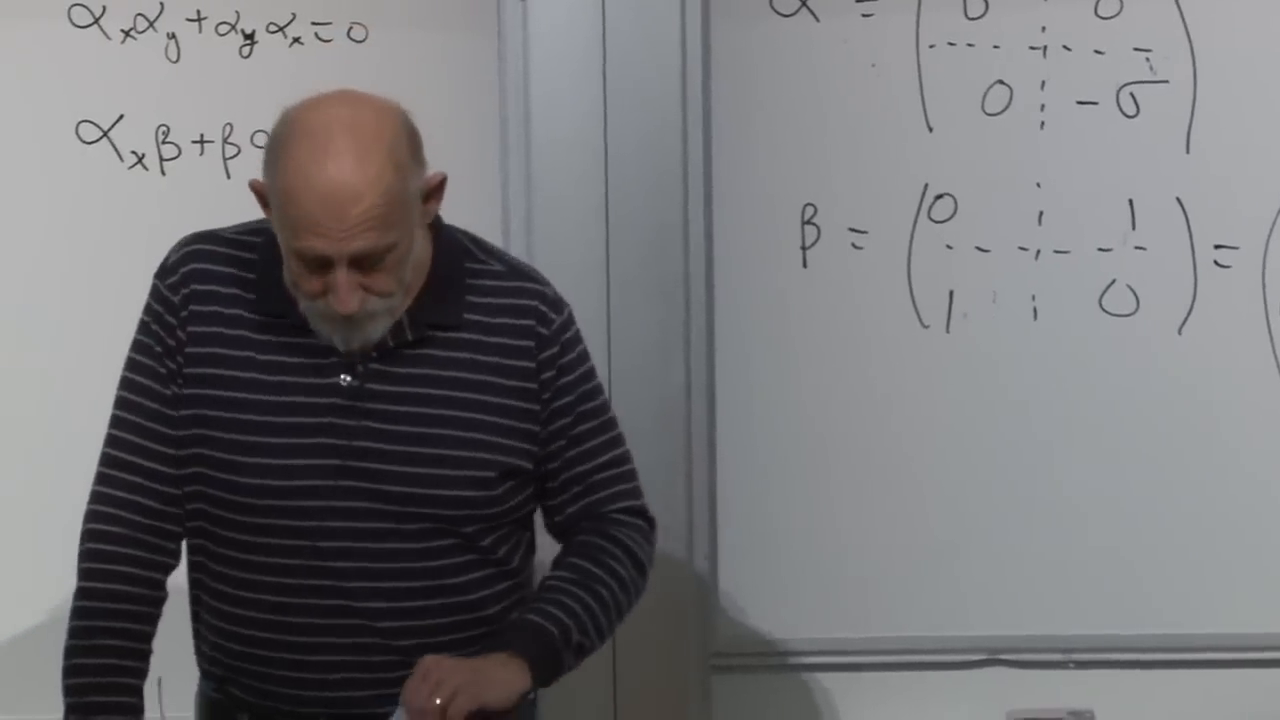
\includegraphics[width=0.94\linewidth]{lecture_10_figure_06.png}
\caption{黑板上的\(4\times4\)分块表示。上面的方程记录了所需的反对易关系；完整矩阵排版于式~\eqref{eq:l10-block-representation}中。}
\lectureframe{00:41:10}
\end{figure}

有质量的哈密顿量现在是
\begin{equation}
H=\boldsymbol{\alpha}\cdot\mathbf P+\beta m
=
\begin{pmatrix}
\boldsymbol{\sigma}\cdot\mathbf P&mI_2\\
mI_2&-\boldsymbol{\sigma}\cdot\mathbf P
\end{pmatrix}.
\label{eq:l10-massive-dirac}
\end{equation}
利用式~\eqref{eq:l10-dirac-algebra}，
\begin{equation}
H^2=\mathbf P^2+m^2.
\end{equation}
因此，四分量结构并不是可有可无的修饰。它是在保持方程一阶的同时，既允许三维动量又允许质量项的最小结构。

\section{手征性与额外分量的意义}

这种扩大添加了什么物理区分？从无质量的上分块开始，
\begin{equation}
H_R=\boldsymbol{\sigma}\cdot\mathbf P,
\end{equation}
以及无质量的下分块，
\begin{equation}
H_L=-\boldsymbol{\sigma}\cdot\mathbf P.
\end{equation}
对于正能态，第一个的自旋与动量同向，第二个的自旋与动量反向。这些是相反的手征性。在无质量理论中，手征性在固有洛伦兹变换下不变，因为没有观察者能够超过一个类光粒子并反转其动量而保持其自旋不变。因此这两个分块描述相反的手征扇区。

\begin{classroomqa}
\lecturetimestamp{00:41:28}
\audiencequestion{在一维中，需要额外的二值自由度来引入质量。在三维中，对应的物理区分是什么？}
\lecturerresponse{它是旋量的手性。两个\(2\times2\)分块携带相反的自旋与动量关系。一个是右手的，另一个是左手的。\(4\times4\)理论包含两者。}
\end{classroomqa}

式~\eqref{eq:l10-massive-dirac}中的质量项是非对角的。它把上分块的振幅送入下分块，反之亦然：
\begin{equation}
\beta m
\begin{pmatrix}
\Psi_R\\
\Psi_L
\end{pmatrix}
=
m
\begin{pmatrix}
\Psi_L\\
\Psi_R
\end{pmatrix}.
\end{equation}
因此质量是相反手征性之间的耦合。

\begin{classroomqa}
\lecturetimestamp{00:43:58}
\audiencequestion{无质量粒子能改变手征性吗？}
\lecturerresponse{在此处展示的自由无质量哈密顿量中不能。两个分块是解耦的，所以一个开始时为右手或左手的状态会保持如此。非对角质量项正是在\(m\ne0\)时混合它们的因素。}
\end{classroomqa}

这种说法对于分块表示是精确的，但不应该把粒子在两个箭头之间机械地翻转这一图像推得太远。物理陈述是波动方程中的矩阵耦合。

\begin{classroomqa}
\lecturetimestamp{00:44:50}
\audiencequestion{这些矩阵是内建于四元数中的吗？}
\lecturerresponse{泡利矩阵与四元数单位密切相关：矩阵\(-i\sigma_i\)的平方为\(-\mathbb{1}\)，并按四元数模式相乘，只差取向约定。完整的狄拉克矩阵需要更大的克利福德代数，而接下来的论证并不需要四元数的联系。}
\end{classroomqa}

\begin{classroomqa}
\lecturetimestamp{00:46:34}
\audiencequestion{如果自旋是角动量，那么这里是否存在与它相关的独立能量项？}
\lecturerresponse{并没有添加任何独立的自由粒子项。旋量结构已经通过矩阵进入动能哈密顿量。将自旋与外磁场耦合会引入额外的相互作用项，但那是另一个问题。}
\end{classroomqa}

\section{{\proseunicodefont α}矩阵是速度，而非自旋}

每个\(\alpha_i\)都有两个\(+1\)本征值和两个\(-1\)本征值。不同分量互不对易，因此它们不能同时被精确测量。要确定其中一个分量代表什么，需使用海森堡方程。对于不含显式时间依赖的算符\(L\)，
\begin{equation}
\dot L=i[H,L].
\label{eq:l10-heisenberg}
\end{equation}
这里的符号约定由Schr\"odinger演化\(e^{-iHt}\)固定。

将式~\eqref{eq:l10-heisenberg}应用于位置算符\(x\)。这些矩阵作用于旋量指标并与位置对易，而只有\(P_x\)不与\(x\)对易：
\begin{align}
\dot x
&=i[\boldsymbol{\alpha}\cdot\mathbf P+\beta m,x]\\
&=i\alpha_x[P_x,x]\\
&=\alpha_x,
\label{eq:l10-velocity}
\end{align}
因为\([P_x,x]=-i\)。因此\(\alpha_x\)是速度算符的\(x\)分量；类似地，
\begin{equation}
\dot{\mathbf x}=\boldsymbol{\alpha}.
\end{equation}

\begin{classroomqa}
\lecturetimestamp{00:51:50}
\audiencequestion{速度分量的测量真的只给出\(+1\)或\(-1\)吗？}
\lecturerresponse{是的，对于以\(c=1\)为单位的瞬时算符\(\alpha_i\)而言。一般态不必是本征态，因此其期望值可以位于这些值之间的任意位置。当粒子有质量时，平滑输运的波包具有低于光速的平均速度。}
\end{classroomqa}

速度不守恒：
\begin{equation}
\dot\alpha_x=i[H,\alpha_x]\ne0.
\end{equation}
含有\(\alpha_y\)、\(\alpha_z\)和\(\beta\)的项不与\(\alpha_x\)对易。因此，同时包含正能分量和负能分量的态会对其位置表现出快速振荡贡献。这就是\emph{zitterbewegung}，字面意思是颤动运动。

在对远长于快速振荡的时间取平均后，预期的相对论速度为
\begin{equation}
\overline{\mathbf v}=\frac{\mathbf p}{E},
\end{equation}
对于慢速电子，它约化为\(\mathbf p/m\)。

\begin{classroomqa}
\lecturetimestamp{00:54:40}
\audiencequestion{自由电子在没有外力的情况下颤动，是否违反牛顿定律？}
\lecturerresponse{不违反。平移不变性使动量守恒，因此\(\dot{\mathbf P}=0\)。狄拉克速度算符并不简单地是\(\mathbf P/m\)，其快速振荡部分可以在动量保持固定的同时发生变化。时间平均后的运动遵循预期的自由粒子关系。}
\end{classroomqa}

\begin{classroomqa}
\lecturetimestamp{00:55:22}
\audiencequestion{速度总是\(c\)吗？}
\lecturerresponse{对某个\(\alpha_i\)的瞬时测量具有本征值\(\pm c\)，但有质量的波包一般是叠加态，其期望值低于光速。其平均群速度为\(\mathbf p/E\)。}
\end{classroomqa}

\begin{classroomqa}
\lecturetimestamp{00:55:30}
\audiencequestion{能否把这种振荡想象成质量使速度发生变化？}
\lecturerresponse{不能。质量是一个固定参数。这种振荡来自速度算符与哈密顿量算符的不对易，或者等价地说，来自能量扇区之间的干涉，而不是来自质量涨落。}
\end{classroomqa}

\begin{classroomqa}
\lecturetimestamp{00:56:22}
\audiencequestion{瞬时测量能否发现速度指向一个方向，而平均运动却指向另一个方向？}
\lecturerresponse{能。该分量算符具有两个精确本征值，而重复测量或时间平均测量则恢复较平滑的漂移。}
\end{classroomqa}

自旋这个词也必须谨慎使用。\(\alpha_i\)作为速度的分量变换，是一个普通矢量。在此表示中，真正的自旋算符是
\begin{equation}
\mathbf S=\frac12\boldsymbol{\Sigma},
\qquad
\Sigma_i=
\begin{pmatrix}
\sigma_i&0\\
0&\sigma_i
\end{pmatrix}.
\label{eq:l10-spin-operator}
\end{equation}
它与\(\alpha_i\)的区别在于下块的符号。这些矩阵密切相关，但速度和自旋不是同一个可观测量。

\section{负能量与最低能量真空}

负能量问题在任何这套矩阵机制出现之前就已经存在。回到一维右行态，
\begin{equation}
H=P.
\end{equation}
由于\(p\)取遍整个实轴，\(E=p\)没有下界。

真空不能仅仅意味着没有粒子的态。它必须是不能从中再移走任何能量的态。如果一个空态允许我们添加一个负能量粒子、降低能量、再添加一个、并无限继续下去，那么这个空态就不是稳定真空。

费米统计提供了一条历史性的出路。在每个负能态中放置一个电子。每加入一个电子都会降低总能量，但泡利不相容原理只允许每个单粒子态中有一个电子。一旦所有负能态都被填满，就没有额外的电子能够落入该区域。狄拉克将这种被填满的组态认定为真空。

同样的构造对玻色子会失败。任意多个玻色子可以占据同一个态，因此一个负能玻色子模式可以无限制地吸收粒子。讲座开始时引入的费米子约束\(n=0,1\)，正是阻止这种下降的东西。

\begin{figure}[htbp]
\centering
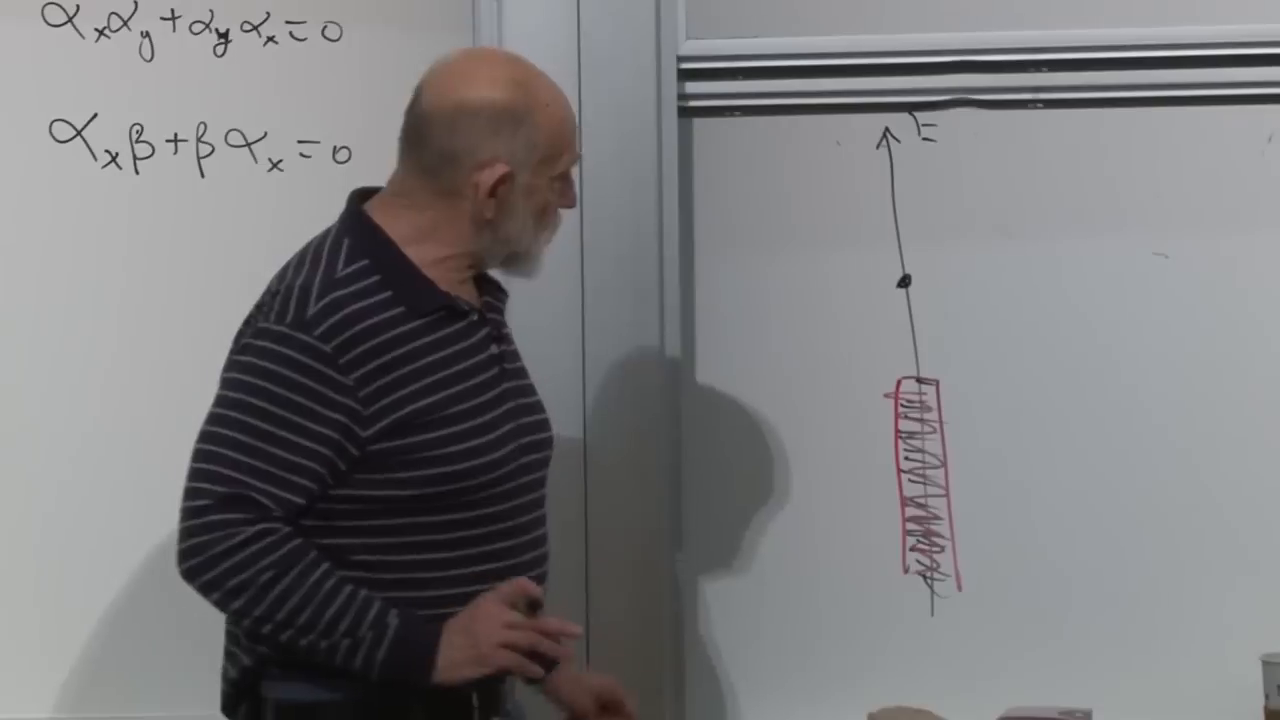
\includegraphics[width=0.94\linewidth]{lecture_10_figure_07.png}
\caption{黑板上历史性的狄拉克海图像：一排负能级被填满直到分界线，正能态位于其上方。}
\lectureframe{01:02:45}
\end{figure}

\begin{figure}[htbp]
\centering
\begin{adjustbox}{max width=\linewidth}
\begin{tikzpicture}[x=1.05cm,y=0.72cm,>=Latex]
\draw[->] (0,-4.8) -- (0,4.8) node[above] {$E$};
\draw[thick] (-2.9,0) -- (3.2,0) node[right] {$E=0$};
\foreach \y in {-4,-3.3,...,-0.5} {
  \draw (-2.3,\y) -- (2.3,\y);
  \foreach \x in {-1.8,-1.2,...,1.8} {
    \fill[blue!65!black] (\x,\y) circle (1.6pt);
  }
}
\foreach \y in {0.8,1.6,...,4.0} {
  \draw (-2.3,\y) -- (2.3,\y);
}
\draw[red,very thick] (0.6,-2.6) circle (5pt);
\draw[red,->,very thick] (0.6,-2.35) .. controls (1.4,-0.4) and (1.2,1.6) .. (1.5,2.4);
\fill[red] (1.5,2.4) circle (2.5pt);
\node[right,red] at (0.85,-2.6) {hole};
\node[right,red] at (1.7,2.4) {$e^-$};
\node[left] at (-2.5,-2.2) {filled negative-energy states};
\end{tikzpicture}
\end{adjustbox}
\caption{对被填满的海之上的激发的一种清晰重构：将一个负能电子激发出来，留下一个正能空穴。}
\end{figure}

海图像是对一种正确的算符重排的历史性说法。其字面上的无限电荷和能量不应被误认为可直接观测的量；现代的重述将消除想象有实物电子填满空间的需要。

\section{空穴是正电子}

当所有负能态都被占据时，有两种激发是可能的。我们可以在海之上添加一个正能电子。或者我们可以移除一个负能电子，留下一个空穴。

空穴具有与被移除电子相反的电荷。移除电荷\(-e\)会使电荷改变\(+e\)。它也具有正的激发能。如果被移除的电子具有\(E_-<0\)，那么相对于被填满的真空测得的能量改变为
\begin{equation}
E_{\mathrm{hole}}=-E_->0.
\end{equation}
空穴是一种正能、带正电的激发：正电子。

一个光子可以将海中的一个电子激发到正能态。相对于真空，末态包含一个电子和一个正电子。在时间有序图中，按惯例将电子的电子数流向上绘制，而正电子线则用相反的箭头。这些箭头追踪的是费米子数或电荷流；它们不是小的经典速度矢量。

\begin{classroomqa}
\lecturetimestamp{01:05:14}
\audiencequestion{这个图像是否要求电子和正电子的数量相等？}
\lecturerresponse{对于任意态来说并不要求。从真空出发并产生一个中性对会各得到一个，但一个态可能已经包含多余的电子或多余的正电子。电荷守恒约束反应；它并不要求每个允许的态都具有相等的粒子数。}
\end{classroomqa}

狄拉克最初并不知道空穴会是一种质量与电子相同、仅在电荷和其他可加量子数上相反的粒子。方程和空穴构造在正电子被纳入熟悉的粒子目录之前就导致了这一预言。

\section{一个费米子场同时包含电子和正电子}

场算符将历史图像带入现代代数。暂时忽略旋量指标、归一化因子和时间依赖。一维场可以示意性地展开为
\begin{equation}
\psi(x)
\sim
\int_{-\infty}^{\infty}dp\,a(p)e^{ipx}.
\label{eq:l10-full-field-integral}
\end{equation}
对于右行色散关系\(E=p\)，正的\(p\)标记正能，负的\(p\)标记负能。将积分拆分：
\begin{equation}
\psi(x)
\sim
\int_0^\infty dp\,a(p)e^{ipx}
+
\int_{-\infty}^0 dp\,a(p)e^{ipx}.
\end{equation}
在第二项中令\(p=-q\)，其中\(q>0\)，并将对填满的负能电子的湮灭重新解释为正电子的产生：
\begin{equation}
b^\dagger(q):=a(-q).
\end{equation}
于是
\begin{equation}
\psi(x)
\sim
\int_0^\infty dp\,
\left[
a(p)e^{ipx}
+
b^\dagger(p)e^{-ipx}
\right].
\label{eq:l10-electron-positron-split}
\end{equation}
平面波相位的精确符号取决于时空约定；不变的内容是\(\psi\)包含一个电子湮灭算符和一个正电子产生算符。

\begin{figure}[htbp]
\centering
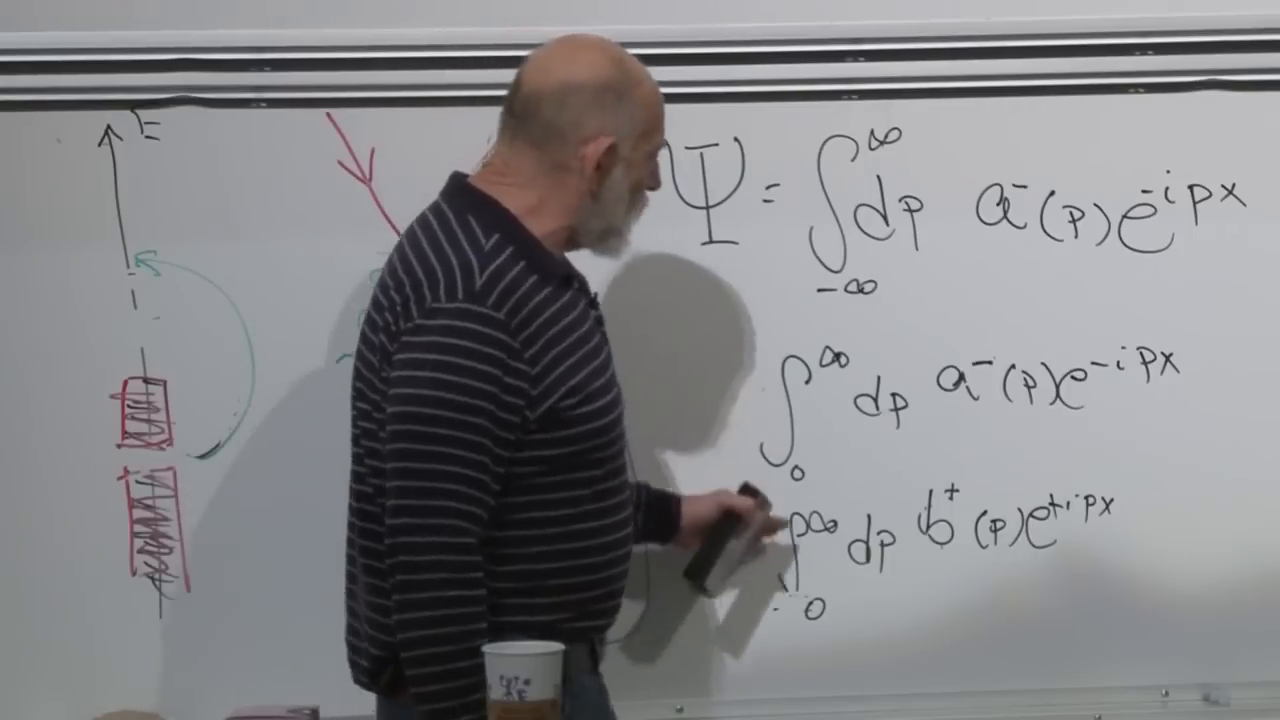
\includegraphics[width=0.94\linewidth]{lecture_10_figure_08.png}
\caption{场积分被拆分为正能区和负能区。下面一行将负能电子算符重新标记为正电子产生算符。}
\lectureframe{01:11:35}
\end{figure}

这正是式~\eqref{eq:l10-fermion-mode}的填满-空对称性发挥作用之处。对于费米子，算符代数允许这种重新标记而不改变其反对易结构。

一个示意性的电磁相互作用具有如下形式
\begin{equation}
H_{\mathrm{int}}
\sim
\int dx\,\psi^\dagger(x)\psi(x)A(x),
\label{eq:l10-qed-schematic}
\end{equation}
其中\(A\)表示光子场。由于每个费米子场都包含电子和正电子两部分，单个局域算符就包含了若干通道：
\begin{align}
e^-&\longrightarrow e^-+\gamma,\\
e^-+e^+&\longrightarrow\gamma,\\
\gamma&\longrightarrow e^-+e^+,
\end{align}
以及它们的逆过程和交叉过程。能量-动量守恒决定在特定环境中哪个通道在运动学上是可能的。例如，真空中一个孤立的实光子不能产生电子-正电子对，除非有另一个参与者来吸收反冲，尽管该局域顶点在相互作用中确实存在。

\begin{figure}[htbp]
\centering
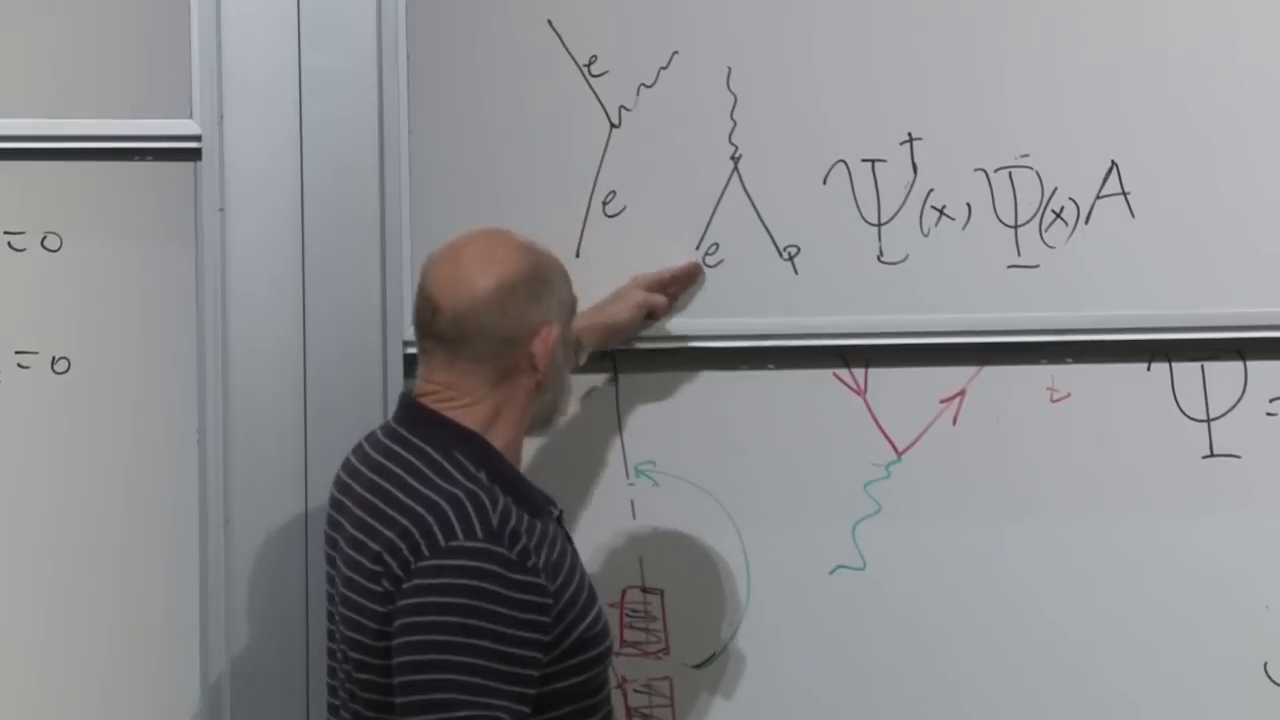
\includegraphics[width=0.94\linewidth]{lecture_10_figure_09.png}
\caption{黑板上并置了电子发射、电子对湮灭以及示意性相互作用\(\psi^\dagger\psi A\)。从同一组场算符中作出不同的选择就产生不同的通道。}
\lectureframe{01:13:30}
\end{figure}

因此，一个紧凑的场乘积就组织起了许多表面上不同的反应。费曼后来给出了用于计算振幅的系统化图解规则，但算符结构的大部分内容在这里已经可见。

\section{现代真空语言与费米海类比}

\begin{classroomqa}
\lecturetimestamp{01:14:20}
\audiencequestion{现代物理学家如何在不把真空当作字面意义上的狄拉克海的情况下描述这一点？}
\lecturerresponse{他们直接进行算符重新解释。负能量电子的湮灭被重新命名为正能量正电子的产生，而真空被定义为被所有电子和正电子湮灭算符湮灭的态。由此得到的表述在粒子与反粒子之间是对称的，并且不需要物质性的海。}
\end{classroomqa}

历史上的海仍然有用，因为其逻辑与凝聚态物质中的情形有密切的类比。在晶体中，固定数目的电子填充最低的可用单粒子态，直到费米能级。被填充的基态并不是空的。把一个电子激发到该能级之上，就会在其下方留下一个未被占据的态。相对于被填充的背景，这个空穴携带正的激发能，并且可以表现得像一个正电荷载流子。

存在重要的差别。固体中的空穴生活在介质中，其有效质量和电荷响应依赖于能带结构。正电子则是相对论量子场中的一种基本反粒子。即便如此，共同的粒子-空穴代数仍使这一类比很有力。

\begin{classroomqa}
\lecturetimestamp{01:17:14}
\audiencequestion{玻色子的克莱因--戈尔登理论是否也会同样地级联到负能量态？}
\lecturerresponse{不会。经过正确量子化的复克莱因--戈尔登场被组织成正能量粒子和反粒子，而不需要填充玻色子海。它的二阶方程和正则结构与狄拉克哈密顿量的构造不同，因此历史上的费米子海论证不能原封不动地搬过来。}
\end{classroomqa}

\begin{classroomqa}
\lecturetimestamp{01:17:30}
\audiencequestion{玻色子的自旋为1是从哪里来的？}
\lecturerresponse{不是来自这里所用的泡利矩阵线性化。自旋为1的场有其自身的洛伦兹变换律和场方程。目前的推导解释的是狄拉克费米子的旋量结构，而不是所有可能的粒子自旋。}
\end{classroomqa}

\begin{classroomqa}
\lecturetimestamp{01:17:46}
\audiencequestion{为什么费米统计对负能量解是必不可少的？}
\lecturerresponse{因为泡利不相容原理把每个态限制为一个电子。一旦所有负能量态都被占据，就没有电子还能落入其中。玻色子的占据没有这样的上限，因此字面意义上的负能量玻色子海仍然没有底。}
\end{classroomqa}

\begin{classroomqa}
\lecturetimestamp{01:20:02}
\audiencequestion{电子与正电子的区别是否只是另一个二值自由度，就像电荷那样？}
\lecturerresponse{从态计数的角度看，有质量的狄拉克场有两个电子自旋态和两个正电子自旋态，因此两个二值标签是有用的助记方式。但粒子与反粒子并不是单个电子的一个可独立旋转的内部量子比特：每个电子都带电荷\(-e\)，每个正电子都带电荷\(+e\)，而这一区分是在量子化之后从正频和负频部分中涌现出来的。}
\end{classroomqa}

这个无限大的海引出了最后一个问题。

\begin{classroomqa}
\lecturetimestamp{01:20:54}
\audiencequestion{无限的狄拉克海会产生无限的宇宙学常数吗？}
\lecturerresponse{它揭示了真空能问题。玻色型零点模贡献\(+\tfrac12\hbar\omega\)，而费米型模以相反的符号贡献。当谱匹配时，形式上的相消是可能的，但电子谱与光子谱并不匹配，因此预期会留下巨大的剩余量。没有引力时，哈密顿量的常数平移可以被减去，因为只有能量差才有意义。有引力时，绝对的真空能会产生引力效应，因此这种减法就成为一个物理问题，而不仅仅是记账。}
\end{classroomqa}

最后要回到质量的含义。

\begin{classroomqa}
\lecturetimestamp{01:22:56}
\audiencequestion{关于质量如何联系左手分量与右手分量，我们还能说得更多吗？}
\lecturerresponse{精确的陈述已经包含在哈密顿量中：非对角项\(m\beta\)把一个手征块映射到另一个手征块。任何关于微观翻转的更机械的图像都是可选的，并且不可避免地是不完整的。}
\end{classroomqa}
